\documentclass[12pt,a4paper]{article}
\usepackage{better_poster}
\graphicspath{{images/}}

% ---- fill in from here

% authors
\title{A conflict can be defined as a fight/disagreement/argument between two sides those sides could be two persons, two or more countries or even yourself.}
\author{Max Sepulveda}

% type of poster: [exp]erimental results, [methods], [theory]
% Disclaimer: the original classification had "study" and "intervention" as separate categories. I group them under experimental results.
\newcommand\postertype{exp} % [exp],[methods],[theory]

\begin{document}

% main point of your study
\makefinding{What is a CONFLICT?}

% \makemain{
% }{

% }
% the main text of your poster goes here
\makemain{

\bigskip

    % you can have 1 or 2 columns
    \raggedcolumns
    \begin{multicols}{2}
    
        \section{People}
       A conflict between 2 persons with different opinions.
        
        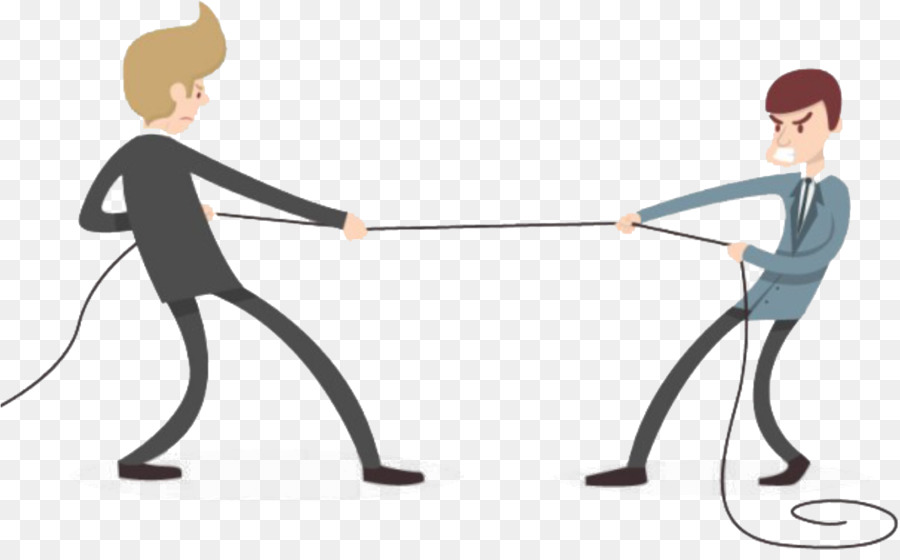
\includegraphics[width=0.8\linewidth]{conflict1.jpg}
            
        \section{Couples}
        A conflict between a couple.

        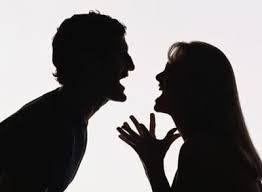
\includegraphics[width=0.8\linewidth]{conflict2.jpg}
        
    % this determines where your columns will be separated
    \columnbreak

       \section{Countries}
       A conflict between two or more countries (war).
       
        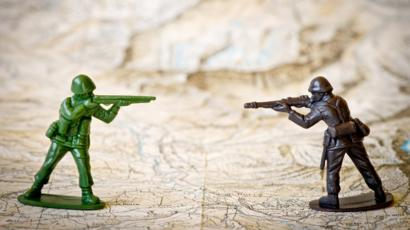
\includegraphics[width=0.8\linewidth]{conflict3.jpg}

       \section{Self}
       A conflict with yourself.
       
        
\includegraphics[width=0.8\linewidth]{conflict4.jpg}
        
    \end{multicols}
}

% footer
% generate qr code from https://www.qr-code-generator.com/ and replace qr_code.png
% default: barcode on the left
\makefooter{LVS_Ascot_arms.jpg}{qr-code-rr.png}

% replace with this like for barcode on the right
%\makealtfooter{images/uni_logo.png}{images/qr-code.png}
 
\end{document}